\documentclass[aspectratio=169]{beamer}
\setbeamertemplate{navigation symbols}{}
\usepackage{color,amsmath,comment, subfigure}
\usepackage{booktabs}
\def\vf{\vfill}
\usepackage{url}

%\setbeameroption{show notes}

%%%%%%%%%%%%%%%%%%%%%%%%%%
\title[]{Lecture 4: Understanding the small world phenomena}
\author[]{Sociology 204: Social Networks, Spring 2021}
\institute[]{Matthew J. Salganik}
\date[]{
1/2: Small world models

\vfill

\begin{flushleft}
\vspace{0.7in}

\includegraphics[width=0.05\textwidth]{figures/cc.png}
\end{flushleft}
}

\begin{document}
%%%%%%%%%%%%%%%%%%%%%%%%%%%
\frame{\titlepage}

\note{
PREFLIGHT:
ask preceptors to sit in back row

FOR NEXT TIME: This was a bit short and didn't include new stuff, perhaps add some of follow-up work
showing that many things are small world
but not everything: http://www.bbc.com/future/story/20131021-the-medieval-facebook-revealed

For next year: y-axis on all graphs is not clear, talk about why scaled values not raw values
}

%%%%%%%%%%%%%%%%%%%%%%%%%%%
\begin{comment}
\begin{frame}

SWBAT:
\begin{enumerate}
\item describe an example where abstract modeling leads to non-intuitive and important insights
\item see an example of similarity of networks across types 
\end{enumerate}

\end{frame}
\end{comment}
%%%%%%%%%%%%%%%%%%%%%%%%
\begin{frame}

Review:
\begin{itemize}
\item empirical vs modeling approaches
\pause
\item empirical approach runs into difficulties
\pause
\item models are different
\pause
\item Erdos-Renyi model is a simple model of networks
\end{itemize}

\pause
Today we will see two different small world models and then an empirical assessment

\note{We left off with the somewhat dead-end in the small world experiments, and so we started to take a turn back to modeling.  The idea of a model is write down some simple rules that we can understand.  Understanding this simple system might help us understand the world.  The point of a model is not to reproduce the world because then it would be as complicated to understand as the world.  The point is to capture the essence of the world as compactly as possible.  In that sense, maybe a model is a bit like poetry: compact essence.

There is something that Duncan left out of the story.  Steve told him that if he works on this problem he should be willing to abandon a job in academia.  And, Duncan did it anyway.  Think about that for a moment.  How many of you want to be doctors?  What if you could explore a problem but that would mean you could never be a doctor?  Would you do it?}

\end{frame}
%%%%%%%%%%%%%%%%%%%%%%%%%
\begin{frame}

Duncan says that they wanted to capture four main ideas:
\begin{itemize}
\item small overlapping groups that are linked by people who belong to multiple groups 
\pause
\item social network evolve
\pause
\item not all relationships are equally likely
\pause
\item occasionally we do things that are not determined by existing network structure
\end{itemize}

\note{
Example of point 1: (e.g., rock climbing and Theoretical and Applied Mechanics Department)\\
Example of point 4: (e.g., Duncan moves from Australia to Cornell)\\
These four ideas look simple but it took them a long time to boil the problem to 4 ideas.\\

Wanted a balance between the forces of structure and agency.   How much do you choose your friends and how much does your environment choose your friends for you?\\
We don't know this balance (in fact we could argue about it forever), instead \textbf{parameterize} to look at many possible worlds.  Explain.\\
}

\end{frame}
%%%%%%%%%%%%%%%%%%%%%%%%%%%%
\begin{frame}

\begin{center}
\includegraphics[width = 0.85\textwidth]{figures_book/3_1}
\end{center}

For mathematical representation, see Eq (5) in Watts (1999)
 
\note{
Caveman world: all friends are friends of friends
Solaria world: make friends randomly
Art as inspiration: The Caves of Steel by Issac Asimov
Next Year: Do a better job explaining this, perhaps add a figure showing two people with varying number of friends in common
}

\end{frame}
%%%%%%%%%%%%%%%%%%%%%%%%%%%
\begin{frame}

\begin{center}
\includegraphics[width = 0.85\textwidth]{figures_book/3_2}
\end{center}

\note{
parameterize
\textbf{Question as technology changes do you think we are moving more toward a (1) caveman world or (2) a solaria world?}
}

\end{frame}
%%%%%%%%%%%%%%%%%%%%%%%%%%%
\begin{frame}

\begin{center}
\includegraphics[width = 0.55\textwidth]{figures_book/3_2}
\end{center}

As technology changes do you think we are moving more toward:
\begin{enumerate}
\item caveman world ($\alpha = 0$)
\item solaria world ($\alpha \rightarrow \infty$)
\end{enumerate}

\end{frame}
%%%%%%%%%%%%%%%%%%%%%%%%%%%
\begin{frame}

\begin{center}
\includegraphics[width = 0.55\textwidth]{figures_book/3_2}
\end{center}

As technology changes do you think we are moving more toward:
\begin{enumerate}
\item caveman world ($\alpha = 0$)
\item \textcolor{blue}{solaria world ($\alpha \rightarrow \infty$)}
\end{enumerate}

\end{frame}
%%%%%%%%%%%%%%%%%%%%%%%%%%%
\begin{frame}

First metric:\\
Characteristics path length $L$: number of edges in shortest path, averaged over all paths\\

\begin{center}
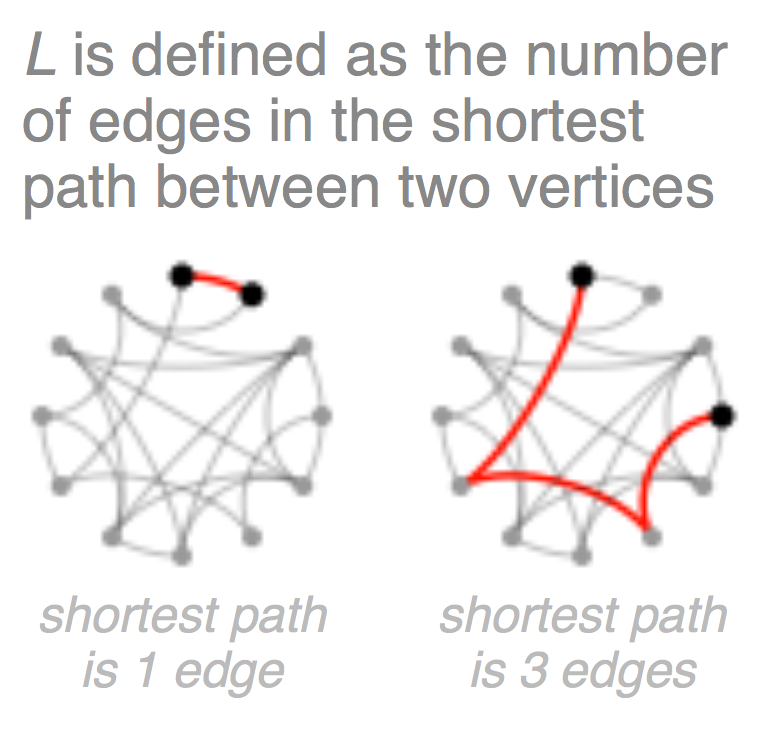
\includegraphics[width = 0.5\textwidth]{figures/victor_2011_L}
\end{center}

\note{One could also write down this down more mathematically}

\end{frame}
%%%%%%%%%%%%%%%%%%%%%%%%%%%
\begin{frame}

Second metric:\\
Clustering coefficient $C$: probability that a two friends of a randomly chosen person are friends\\

\begin{center}
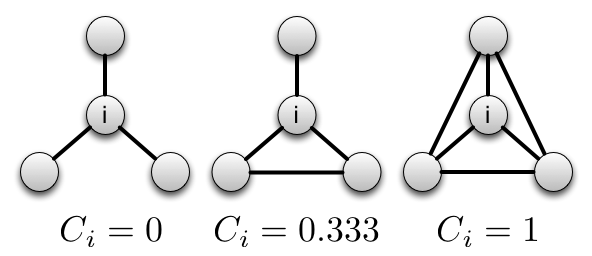
\includegraphics[width = 0.5\textwidth]{figures/local_clustering_coeff}
\end{center}

\note{One could also write down this down more mathematically}

\end{frame}
%%%%%%%%%%%%%%%%%%%%%%%%%%%%%%
\begin{frame}

\begin{center}
\includegraphics[width = 0.85\textwidth]{figures_book/3_4}
\end{center}

\note{Simulate lots of people following these rules?  What happens?}

\end{frame}
%%%%%%%%%%%%%%%%%%%%%%%%%%%
\begin{frame}

\begin{center}
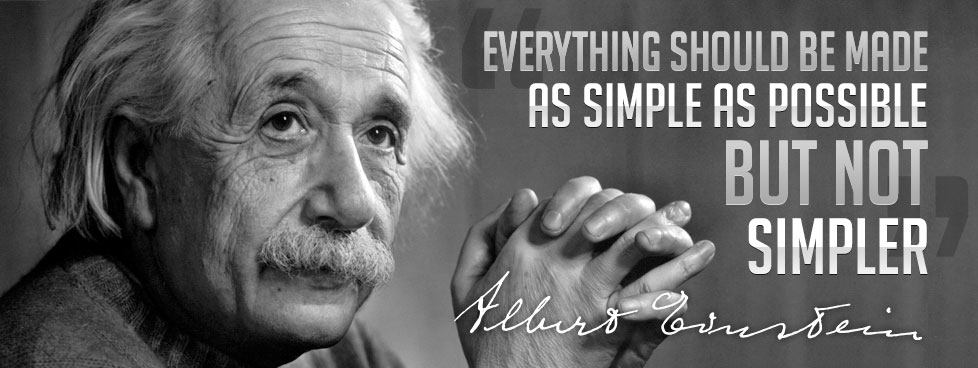
\includegraphics[width = 0.95\textwidth]{figures/einstein_everything_simple}
\end{center}

\tiny{\url{http://vireomd.net/blog/dhc/einstein-kiss.html}}

\note{This seems promising, but it is too complicated.  What is $\alpha$?  What should be the substrate (described in AJS article)?  But not only is it too complicated, it is too simple (it leaves many key facts).  Rather than getting more complicated they decided to get more simple.  This is the magic.
}

\end{frame}
%%%%%%%%%%%%%%%%%%%%%%%%%%%
\begin{frame}

\begin{center}
\includegraphics[width = 0.85\textwidth]{figures_book/3_6}
\end{center}

\end{frame}
%%%%%%%%%%%%%%%%%%%%%%%%%%%
\begin{frame}
\frametitle{}

\begin{center}
\includegraphics[width = 0.85\textwidth]{figures_book/3_7}
\end{center}

\note{Very simple tradeoff between order and randomness.  Average path length changes fast, clustering coefficient changes slowly. The key insight though is \textbf{shortcuts}: adding one edge can change the average path length for many people (a friendship between Duncan and someone at Cornell reduces the path length between many people in Australia and many people in the US).
Small imperceptible changes at the local level lead to big changes at the global level.
Adding just 5 shortcuts reduces the average path length in half (watts, 1999) p 89
}

\end{frame}
%%%%%%%%%%%%%%%%%%%%%%%%%%%%%%%
\begin{frame}

Demo:
\url{http://mathinsight.org/small_world_network}

\end{frame}
%%%%%%%%%%%%%%%%%%%%%%
\begin{frame}

\begin{center}
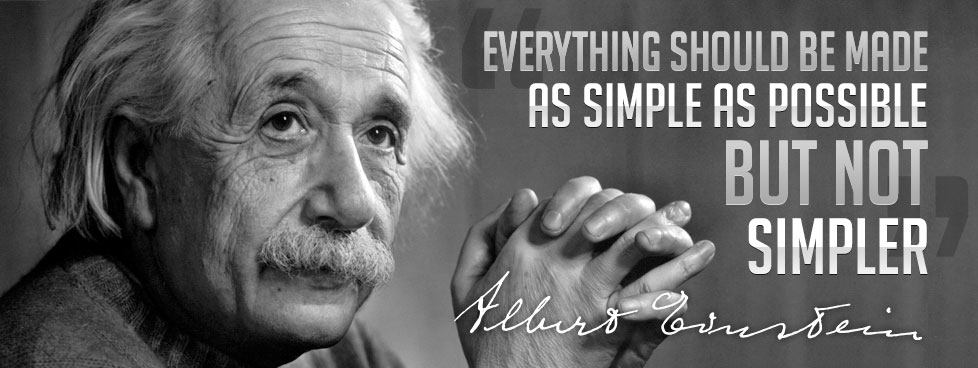
\includegraphics[width = 0.95\textwidth]{figures/einstein_everything_simple.png}
\end{center}

\tiny{\url{http://vireomd.net/blog/dhc/einstein-kiss.html}}

\note{\textbf{LESS realistic model yields MORE insight}.  This is very rare.  It almost never happens.  In some sense this is what every scientist is hoping for.\\
because model is so general it suggests that ``small worlds'' may exist in other types of networks.  This is key.  Only because the model was so simple (and so general) would it lead to thoughts about small worlds in other types of networks.  \\

Another benefit of simplicity is that it suggests connections to other areas.  Given this result, why just social networks?  Why not any ordered network with some randomness?}

\end{frame}
%%%%%%%%%%%%%%%%%%%%%%%%%%%
\begin{frame}
\frametitle{}

Are real networks small world networks?

\begin{center}
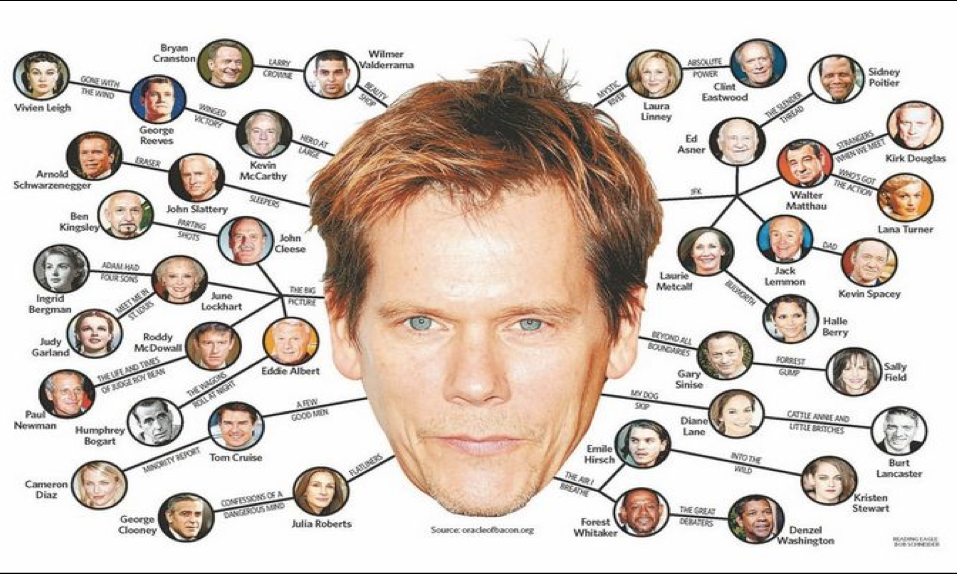
\includegraphics[width = 0.7\textwidth]{figures/degrees_of_bacon}
\end{center}

\end{frame}
%%%%%%%%%%%%%%%%%%%%%%%%%%%

\end{document}
